\chapter{Results}
\label{chap:results}

This chapter presents the physiological and behavioural outcomes of the study.
Results are organised into three parts:
(a) heart-rate variability (HRV) during meditation,
(b) within-group changes between the stress and meditation phases, and
(c) between-group comparisons of these changes for Conventional versus VR meditation.

Statistical tests were selected based on distributional assumptions assessed for
each variable. Within-group comparisons (stress vs.\ meditation) were conducted
using paired-samples \textit{t}-tests when normality was met; otherwise, Wilcoxon
signed-rank tests were applied. Between-group comparisons were performed using
independent-samples \textit{t}-tests or Mann--Whitney~$U$ tests on change scores
($\Delta = \text{Meditation} - \text{Stress}$). Non-significant results are reported
as \textbf{ns} ($p > 0.05$).

\noindent\textbf{Group definitions.}
Participants in the VR condition were asked to report their perceived stress level
(high or low) when prompted by the AI at the beginning of the VR session.
Based on this self-reported stress level, the VR sample was divided into two
exploratory subgroups: \textit{VR--HighStress} and \textit{VR--LowStress}.
This subdivision reflects subjective stress perception rather than physiological
criteria and was used for descriptive and exploratory analyses only.
The \textit{Conventional} group completed the same experimental procedure
without VR and without subgrouping. The VR–HighStress and VR–LowStress labels therefore describe subjective stress perception at session start and should not be interpreted as objective physiological stress categories.


\section{Heart-Rate Variability During Meditation}
\label{sec:results_hrv}

Heart-rate variability (HRV) metrics were extracted from BVP signals during the 240\,s
meditation period.
The key indices included mean heart rate (HR), SDNN (overall HRV), RMSSD (short-term parasympathetic
activity), pNN50 (beat-to-beat vagally modulated variability), and LF/HF ratio (sympathovagal balance). For completeness, the full set of HRV summary statistics is provided in Table~\ref{tab:hrv-summary}.

\begin{table}[H]
    \centering
    \caption{Group means (SD) for HRV metrics during the meditation phase.}
    \label{tab:hrv-summary}
    \begin{tabular}{lccccc}
        \toprule
        \textbf{Group} & \textbf{HR (bpm)} & \textbf{SDNN (s)} & \textbf{RMSSD (s)} & \textbf{pNN50 (\%)} & \textbf{LF/HF} \\
        \midrule
        Conventional & 97.95 (23.00) & 0.146 (0.052) & 0.187 (0.074) & 53.60 (15.81) & 0.94 (0.61) \\
        VR High Stress     & 111.90 (25.31) & 0.119 (0.043) & 0.141 (0.043) & 52.11 (16.45) & 0.85 (0.41) \\
        VR Low Stress       & 87.23 (12.30)  & 0.153 (0.098) & 0.179 (0.135) & 48.13 (22.46) & 1.53 (1.38) \\
        \bottomrule
    \end{tabular}
\end{table}

Overall, no statistically significant differences in HRV metrics were observed
between groups during the meditation phase ($p > 0.05$ for all comparisons).
Nevertheless, descriptive trends were physiologically plausible.
Both the Conventional and VR-Low stress conditions exhibited numerically higher SDNN and RMSSD values than the VR-High condition, suggesting relatively stronger
parasympathetic activation and autonomic flexibility.
Mean heart rate was lowest in the VR-Low stress group and highest in the VR-High stress group,
consistent with the subjective subgroup classification, although variability was high.

The LF/HF ratio showed substantial inter-individual variability, particularly in
the VR-Low group, limiting its interpretability in short-duration recordings.
Taken together, these findings indicate that meditation was associated with physiological relaxation across all conditions.
However, HRV metrics did not reliably differentiate between meditation modalities within the time window of this study. It should be noted that reliable interpretation of HRV metrics typically requires longer recording windows ($\geq$
5 minutes) \cite{taskforce1996hrv} than those used in the present protocol, which may have limited sensitivity to subtle between-group differences. Figure~\ref{fig:hrv-metrics} visualises the group-level HRV metrics during the meditation phase.



\begin{figure}[H]
    \centering
    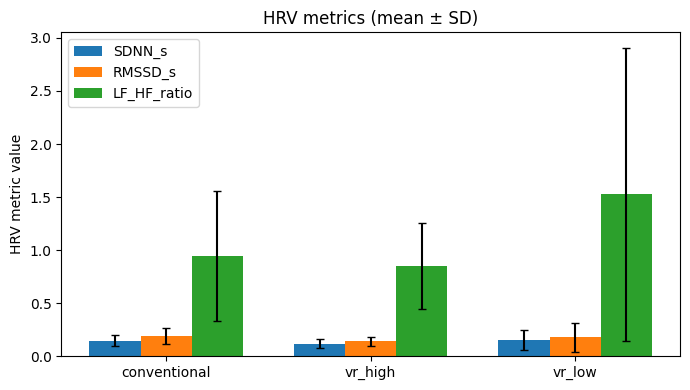
\includegraphics[width=0.85\textwidth]{pics/result plots/new result comparison/HRV MEAN.png}
    \caption{Group-level HRV metrics (mean $\pm$ SD) for the three meditation conditions.}
    \label{fig:hrv-metrics}
\end{figure}

No statistically significant group differences emerged for any HRV metric.
The HRV results are therefore interpreted as descriptive context rather than as primary evidence
for differential effectiveness of the meditation modalities.

\section{Within-Group Changes: Stress vs.\ Meditation}
\label{sec:within}

To evaluate whether meditation induced measurable physiological relaxation,
each group's stress-phase values were compared with their meditation-phase averages.
Table~\ref{tab:within-group} summarises the direction and significance of these changes.

\begin{table}[H]
    \centering
    \caption{Within-group comparisons between stress induction and meditation.
Arrows indicate the direction of change from stress to meditation within each group ($\uparrow$ increase; $\downarrow$ decrease).
``ns'' indicates non-significance ($p > 0.05$). VR-High Stress and VR-Low Stress are exploratory subgroups within the VR condition defined a priori by self-reported stress level.}

    \label{tab:within-group}
    \begin{tabular}{lccccc}
        \toprule
        \textbf{Group} & \textbf{SCL} & \textbf{HR} & \textbf{PVA} & \textbf{TEMP} & \textbf{MOTION} \\
        \midrule
        Conventional & $\uparrow$, $p < 0.001$  & ns & ns & $\uparrow$, $p = 0.013$ & ns \\
        VR High Stress      & ns ($p = 0.065$)         & ns & $\downarrow$, $p = 0.031$ & ns ($p = 0.066$) & ns \\
        VR Low Stress      & $\downarrow$, $p = 0.004$ & ns & ns & $\uparrow$, $p = 0.040$ & $\downarrow$, $p < 0.001$ \\
        \bottomrule
    \end{tabular}
\end{table}

Across all conditions, peripheral skin temperature increased during meditation,
consistent with relaxation-related peripheral vasodilation and reduced sympathetic activity. This pattern indicates that both conventional and VR-based meditation elicited
physiological relaxation at the autonomic level.

Electrodermal responses differed between conditions. The Conventional group showed
a significant increase in tonic skin conductance level (SCL), a pattern commonly
observed in passive seated tasks and likely influenced by electrode drift or
thermoregulatory effects rather than heightened stress. In contrast, the VR-Low
group exhibited a significant decrease in SCL, suggesting stronger sympathetic
down-regulation during VR meditation for participants with lower baseline stress. Figure~\ref{fig:scl-time} shows the group-mean skin conductance level (SCL) over time for the three meditation groups during the meditation phase.



\begin{figure}[H]
    \centering
 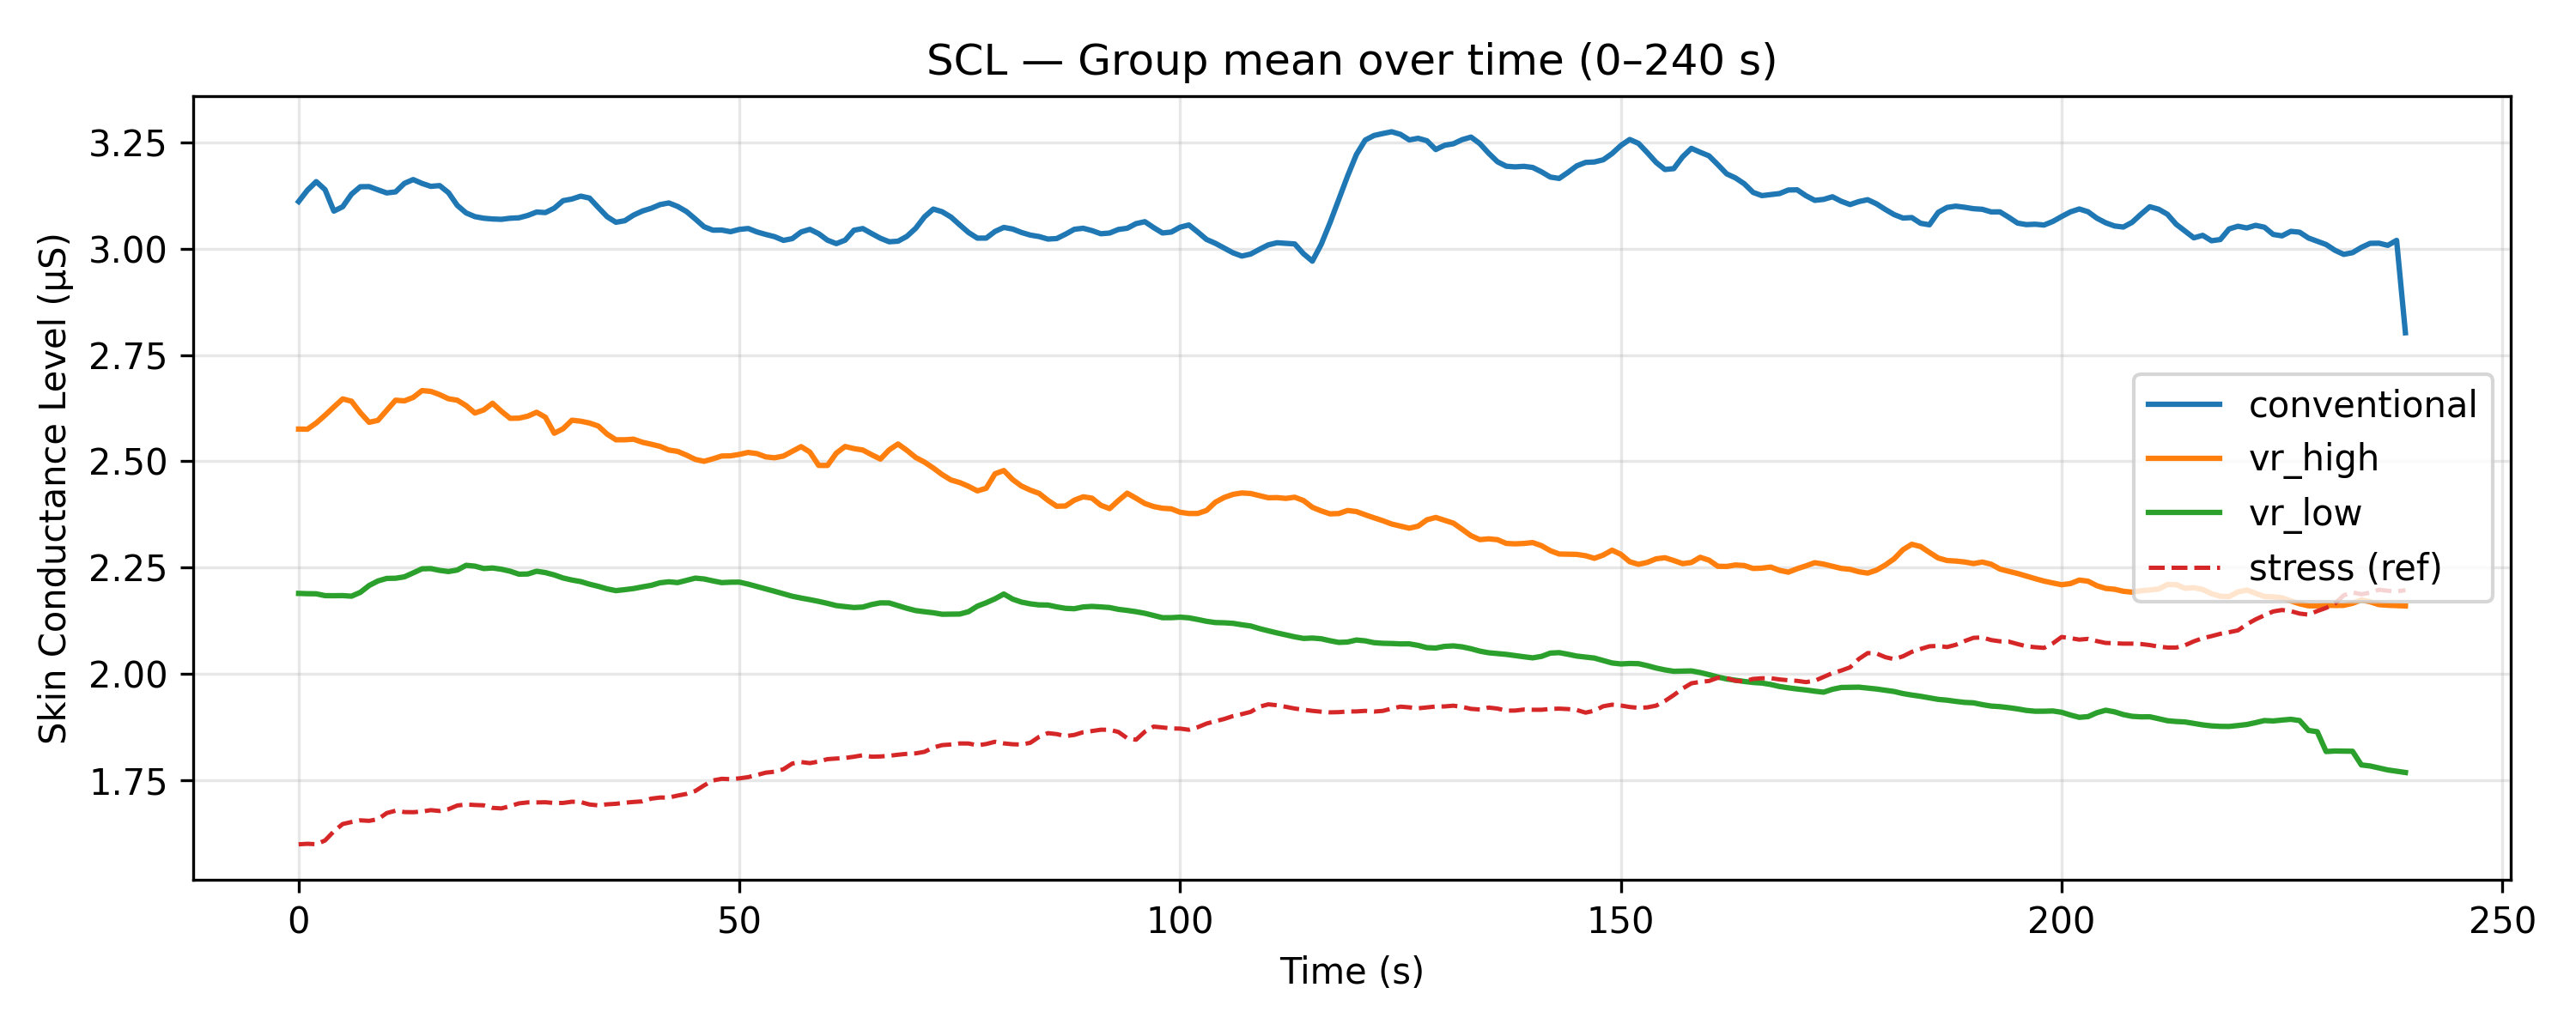
\includegraphics[width=0.85\textwidth]{pics/result plots/timeseries_scl.png}
    \caption{Group-mean SCL over time for all three meditation groups.}
    \label{fig:scl-time}
\end{figure}

Movement amplitude decreased markedly in the VR-Low group ($p < 0.001$), indicating
greater physical stillness and reduced restlessness during meditation. This effect
was not observed in the Conventional group, supporting the interpretation that VR
facilitated deeper bodily engagement and attentional stability.

Heart rate did not change significantly in any group, which is consistent with
prior meditation research showing that short sessions often stabilise rather than
reduce cardiac rate. The reduction in pulse volume amplitude observed in the
VR-High group is interpreted cautiously, as PVA is highly sensitive to breathing
patterns and sensor placement and does not consistently reflect relaxation in
short-duration recordings.


To illustrate the thermal response, Figure~\ref{fig:temp-time-main} shows the group-mean skin temperature for Conventional meditation versus VR meditation, where the VR curve represents the average of the VR–High and VR–Low subgroups, which exhibited comparable
temperature trends.


\begin{figure}[H]
    \centering
    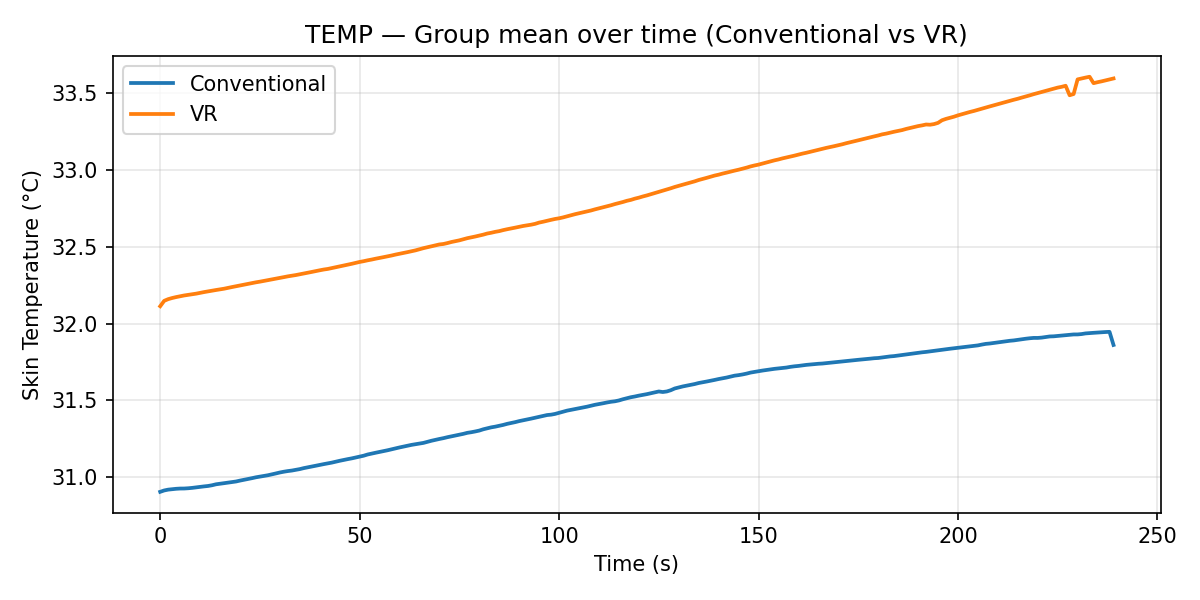
\includegraphics[width=0.85\textwidth]{pics/result plots/lines_collapsed_TEMP.png}
    \caption{Group-mean skin temperature over time for Conventional versus VR.}
    \label{fig:temp-time-main}
\end{figure}

In general, the within-group analyses demonstrate that meditation induced measurable
physiological relaxation across conditions, with VR particularly in the low-stress
subgroup showing clearer markers of autonomic regulation and physical stillness.


\section{Between-Group Differences in Physiological Change}
\label{sec:between}

To determine whether VR meditation produced stronger physiological regulation than conventional
audio meditation, change scores ($\Delta = \text{Meditation} - \text{Stress}$) were compared between
Conventional and VR (with VR-High and VR-Low collapsed).
Table~\ref{tab:between-group} summarises these comparisons.

\begin{table}[H]
    \centering
    \caption{Between-group comparison of change scores ($\Delta$).  
    Only motion amplitude showed a statistically significant difference.}
    \label{tab:between-group}
    \begin{tabular}{lccc}
        \toprule
        \textbf{Signal} & \textbf{Conventional $\Delta$} & \textbf{VR $\Delta$} & \textbf{$p$-value} \\
        \midrule
        SCL    & 0.803  & 0.600   & 0.487 \\
        HR     & -0.096 & -1.256  & 0.708 \\
        PVA    & 3.046  & -4.153  & 0.078 \\
        TEMP   & 0.797  & 1.431   & 0.473 \\
        MOTION & 0.026  & -0.024  & 0.005 \\
        \bottomrule
    \end{tabular}
\end{table}

Figure~\ref{fig:delta-motion} illustrates the significantly lower per-participant motion amplitude observed in the VR condition compared to conventional meditation.
Motion amplitude was the only physiological measure showing a statistically significant
between-group difference. Participants in the VR condition exhibited a greater reduction
in movement compared to the conventional meditation group, indicating enhanced behavioral
stillness and attentional engagement during VR meditation.

\begin{figure}[H]
    \centering
    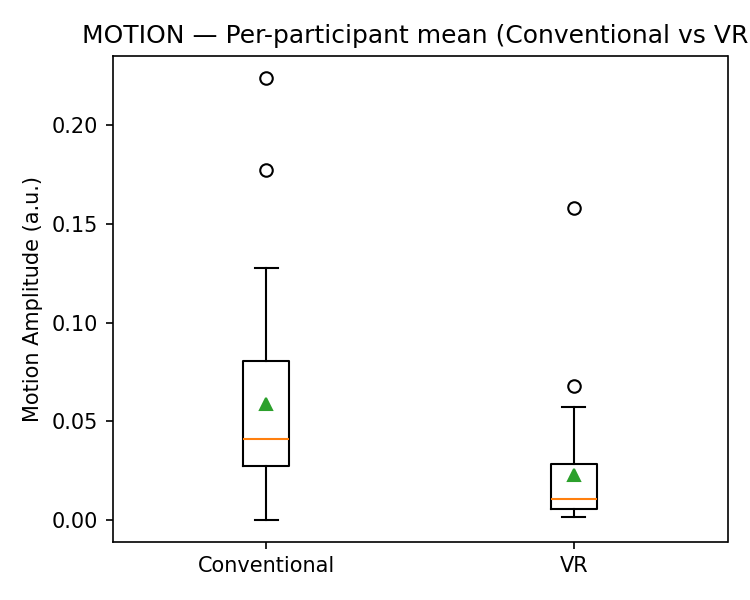
\includegraphics[width=0.85\textwidth]{pics/result plots/box_collapsed_MOTION.png}
    \caption{Per-participant mean motion amplitude for Conventional vs.\ VR.  
    VR resulted in significantly lower motion during meditation ($p = 0.005$).}
    \label{fig:delta-motion}
\end{figure}

All autonomic measures (SCL, HR, PVA, and TEMP) did not differ significantly between modalities ($p > 0.05$). This suggests that, within the duration of the present experiment, VR and conventional meditation induced comparable levels of physiological relaxation.


\section{Questionnaire Results}
\label{sec:questionnaire_results}

A total of 44 valid participants completed the post–study questionnaire
(VR meditation: $n = 23$; conventional meditation: $n = 21$). Due to missing or invalid responses on individual questionnaire items,
the effective sample size for some statistical analyses was reduced,
while descriptive statistics reflect the full number of completed
questionnaires.
The questionnaire assessed baseline perceived stress, pre–post-meditation negative affect, state mindfulness during meditation, perceived presence (VR only), and overall satisfaction with the meditation method.

Table~\ref{tab:questionnaire_descriptives} summarises descriptive
statistics for the main scales by mode of delivery (VR vs.\ conventional
meditation).


% Descriptive table
\begin{table}[t]
  \centering
  \caption{Descriptive statistics (mean $\pm$ SD) for questionnaire scales (1-5 Likert scale; midpoint = 3).}

  \label{tab:questionnaire_descriptives}
  \begin{tabular}{lcccc}
  \toprule
   & \multicolumn{2}{c}{VR meditation} & \multicolumn{2}{c}{Conventional} \\
  \cmidrule(lr){2-3}\cmidrule(lr){4-5}
  Measure & $n$ & $M \pm SD$ & $n$ & $M \pm SD$ \\
  \midrule
  Baseline perceived stress       & 23 & $3.59 \pm 0.89$ & 21 & $3.59 \pm 0.75$ \\
  Negative affect (pre)           & 23 & $2.94 \pm 0.85$ & 21 & $2.79 \pm 0.78$ \\
  State mindfulness               & 23 & $3.42 \pm 0.73$ & 21 & $3.06 \pm 0.89$ \\
  Overall satisfaction            & 23 & $4.09 \pm 0.68$ & 21 & $3.00 \pm 1.27$ \\
  Presence (VR only)              & 23 & $3.38 \pm 0.74$ & -- & -- \\
  \bottomrule
\end{tabular}

\end{table}


\subsection{Baseline Measures}

Before the meditation session, both groups exhibited comparable levels
of baseline perceived stress. A Mann--Whitney $U$ test revealed no
significant difference between VR and conventional meditation
($U = 234.0$, $p = 0.8578$). Similarly, pre-session negative affect did
not differ significantly between groups
($U = 266.5$, $p = 0.5699$).


Together, these results indicate that participants entered the
experiment with similar affective states, reducing the likelihood that
subsequent differences were driven by baseline imbalances.


\subsection{State Mindfulness During Meditation}
Participants in the VR condition reported higher state mindfulness
during meditation than those in the conventional condition
(Table~\ref{tab:questionnaire_descriptives}). However, this difference
did not reach statistical significance, ($U = 267.5$, $p = 0.5558$).

This pattern suggests a tendency for VR meditation to support sustained
attentional focus, although the present sample size does not allow this
effect to be confirmed statistically.


\subsection{Perceived Presence in VR}


Perceived presence was assessed only in the VR condition. Overall, participants reported a clearly positive sense of being ``inside'' the
virtual environment (Table~\ref{tab:questionnaire_descriptives};
$M = 3.38$, $SD = 0.74$ on a 1-5 Likert scale), indicating a moderately positive
sense of presence relative to the neutral midpoint. No equivalent measure was collected in the conventional group; therefore, no direct statistical comparison was possible. Figure~\ref{fig:presence_questionnaire} shows the distribution of presence ratings for participants in the VR meditation condition.


\begin{figure}[t]
  \centering
  
\includegraphics[width=.55\textwidth]{pics/result plots/fig5_presence_VR_only.png}
  \caption[Perceived presence in VR]%
  {Sense of presence ratings for participants in the VR meditation
   condition.}
  \label{fig:presence_questionnaire}
\end{figure}

%--------------------------
\subsection{Overall Satisfaction With the Meditation Method}
%--------------------------
Satisfaction was rated on the same 1-5 Likert scale as the other questionnaire measures.
In contrast to the baseline measures, overall satisfaction differed clearly between groups. Participants in the VR condition reported
substantially higher satisfaction ($M = 4.09$, $SD = 0.68$), which is clearly above the neutral midpoint of the
1-5 scale, than those in the conventional condition
($M = 3.00$, $SD = 1.27$). This effect was statistically significant ($U = 364.0$, $p = 0.0027$), indicating that the VR experience was perceived as more enjoyable and more
worthwhile overall. A Mann-Whitney $U$ test was used due to the ordinal nature of the satisfaction ratings and the independent group design.  Figure~\ref{fig:satisfaction_questionnaire} visualises the distribution of overall satisfaction ratings for VR and conventional meditation conditions.


\begin{figure}[t]
  \centering
  
\includegraphics[width=.55\textwidth]{pics/result plots/fig4_satisfaction_VR_vs_Conventional.png}
  \caption[Overall satisfaction with VR vs.\ conventional meditation]%
  {Overall satisfaction ratings for VR and conventional meditation
   conditions.}
  \label{fig:satisfaction_questionnaire}
\end{figure}

It is worth noting that the VR group included a higher proportion of
meditation-naive participants compared to the conventional group
(Table~\ref{tab:meditation-experience}). This imbalance may have
influenced subjective evaluations such as overall satisfaction and
perceived presence, as participants without prior meditation experience
may perceive guided and immersive VR environments as more novel or
engaging.

\subsection{Differences Within VR: Low- vs.\ High-Stress Subgroups}

VR participants were further categorised into low-stress and high-stress
subgroups based on their self-reported stress level at the beginning of the VR session. Physiological measures were analysed separately to characterise
stress-to-meditation changes within these subgroups. Because the resulting subgroup sizes were small and
unbalanced, no inferential statistical tests were conducted for direct
comparisons between these VR subgroups.

Descriptively, participants in the low-stress subgroup tended to report
slightly higher state mindfulness and a stronger sense of presence than
those in the high-stress subgroup, while overall satisfaction with the
VR meditation experience appeared similarly high across both groups.
These patterns are reported for an exploratory context only.

Accordingly, the observed subgroup differences should be interpreted
with caution and not as evidence of systematic effects. They suggested
that lower physiological stress during VR meditation may be associated
with a marginally enhanced subjective sense of immersion, but this
interpretation remains speculative and would require confirmation in
future studies with larger and statistically powered subgroup samples.



\subsection{Correlations Between Questionnaire Measures}
\label{sec:questionnaire_correlations}

Exploratory associations between questionnaire measures were examined to
identify relationships between subjective stress, affect, mindfulness,
presence, and satisfaction (Figure~\ref{fig:questionnaire_correlations}).
These analyses were intended to provide descriptive insight into how
self-reported experiences co-varied across participants.

Baseline perceived stress and pre-meditation negative affect showed a
strong positive association, indicating that participants who reported
higher stress levels also tended to report higher negative affect before
the meditation session. In addition, state mindfulness during meditation
was positively associated with overall satisfaction, suggesting that
participants who felt more focused and present during the meditation
tended to evaluate the experience more positively.

These associations are descriptive and exploratory in nature and were
not used for confirmatory hypothesis testing.


\section{Summary of Findings}
\label{sec:summary}

The combined analysis of physiological signals and questionnaire responses provides a clearer picture of how VR meditation compares to conventional meditation.

From the physiological perspective, all groups showed indicators of relaxation during the meditation phase. Temperature increased across conditions, and motion generally decreased, with the most pronounced stillness observed in the VR–low group. Heart-rate variability metrics (SDNN, RMSSD, pNN50, LF/HF) did not differ significantly across groups, suggesting that within the short time window of this study VR and conventional meditation elicited comparable autonomic responses.

Skin conductance level showed an increase in several groups, which is likely attributable to finger electrode dynamics rather than genuine sympathetic activation. Importantly, no measure indicated that VR meditation produced higher physiological arousal than the conventional method. Instead, the reduction in motion particularly supports the interpretation that VR encouraged stronger physical stillness and bodily engagement.

The questionnaire results complement and extend these observations. Baseline stress and negative affect were matched between VR and conventional participants, ensuring fair comparability. Although state mindfulness scores were slightly higher in VR, this difference was not statistically significant. In contrast, the sense of presence was markedly higher in VR, reflecting the immersive nature of the virtual environment. Most notably, overall satisfaction was significantly higher in VR than in conventional meditation, indicating that users found the VR-based experience more enjoyable, engaging, and well-guided.

Taken together, the findings show that both VR and conventional meditation produced similar physiological relaxation outcomes, but the VR condition offered clear subjective advantages. Participants reported feeling more present, more engaged, and more satisfied
with the experience, with ratings exceeding the neutral midpoint of the
1--5 response scale. VR appears to enhance the qualitative, experiential dimension of meditation without compromising physiological relaxation and, in some cases, even supporting more consistent stillness.

This integrated interpretation suggests that VR meditation is a viable and appealing alternative to conventional practices, particularly when the goal is to increase engagement, immersion, and user satisfaction while maintaining comparable physiological benefits.

Overall, the results indicate that VR meditation primarily enhances
experiential, behavioral, and subjective dimensions of meditation
(e.g., presence, satisfaction, physical stillness), while short-term
autonomic physiological responses remain comparable to those observed
during conventional meditation.


Additional descriptive figures for all signals are provided in Appendix~\ref{app:supp-figs}.
